This research, in accordance with the goals depicted in the previous
  section, started by considering the collection of spectra of M stars
  provided by DwarfArchives.org, a compendium of L, M and T dwarfs,
  maintained by Chris Gelino, Davy Kirkpatrick and Adam Burgasser.

This choice of dataset determines the search space for optimal
features. We describe its main characteristics in the following
paragraphs.

In principle, we aim at developing a procedure to identify suitable
reference bands for signal and continuum in this particular class of
stars. Simultaneously, we define alternative ways to represent the
spectra and compare their utility in predicting stellar parameters. In
order to have a homogeneous and complete coverage of parameter space,
we decided to use a library of synthetic spectra as the benchmark for
the feature selection. In particular, we chose the BT-Settl library
(\cite{2013MSAIS..24..128A}). 

\subsection{Dataset Selection}
\label{subsec:DS}
 The DwarfArchives M dwarf database includes spectra for over 500 of
  the nearest and brightest M dwarfs in the same wavelength range
  (roughly 6300-9000{\AA})(\cite{Kirkpatrick:2002eh}) with
  spectroscopic observations obtained at the Multiple Mirror Telescope
  (MMT, efective aperture 4.5m) on Mount Hopkins AZ and the McDonald
  Observatory 2.7 telescope on Mount Locke, TX. The spectra from the
  IPAC dataset have no uncertainty defined.

 At the MMT spectra were obtained with a Red Channel Spectrograph
  equipped with an 800x800 TI CCD. A 270 line mm\textsuperscript{-1}
  grating with an LP-945 order blocking filter was used to cover the
  range 6300 - 9000{\AA} at a resolution of 18{\AA}. At McDonald,
  spectra covered the range 6400 - 9200{\AA} at a resolution of
  12{\AA}(\cite{1994AJ....108.1437H}).

\subsection {Library of synthetic spectra}

\label{subsec:RTL}

The actual subset of the BT-Settl used for the feature selection
process covers effective temperatures between 2000 and 4200 K in steps
of 100 K, gravities in the range -6 < \logg < 1 with a step of 0.5
dex, and metallicities relative to solar values equal to 0, -0.5 or -1
dex.

The original BT-Settl spectra were degraded from the original 0.1{\AA}
sampling to the required resolution and sampling of the IPAC
collection of spectra.  Then, spectra were trimmed to produce valid
segments between 6000 and 9150{\AA} and normalised to unit area in
order to place them all in the same scale regardless of its intrinsic
brightness. The total number of spectra meeting our requirements (429)
was rather limited for our purposes, and we decided to interpolate the
mesh. We compared a few PHOENIX \cite{fuhrmeister2005phoenix} models
with our (inverse of the square distance) weighting scheme
interpolations at a few selected points to assess the validity of our
interpolation. The results can be judged from
Fig.~\ref{fig:comp_gen_inter}.


\begin {figure}
 \begin{center}
 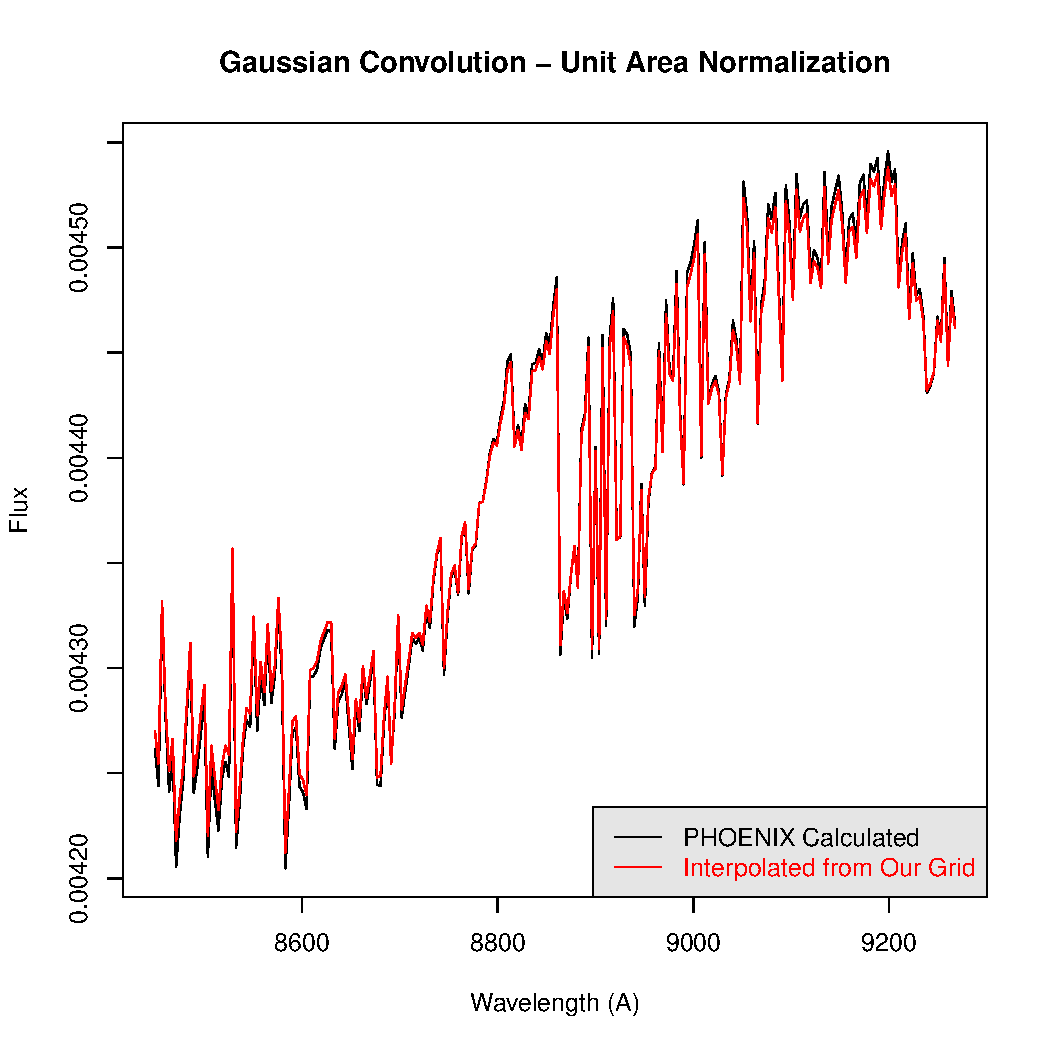
\includegraphics[width=6cm]{figs/intgrid4_gauss.pdf}
 \caption{Comparison between PHOENIX and interpolated spectra}
 \label{fig:comp_gen_inter}
 \end{center}
\end {figure}


Several sets of BT-Settl spectra are produced for grids of different
step sizes. The mesh with 0.25 dex for both \logg and metallicity and
a temperature step of 50K produced a total 1329 spectra.  Another
reinterpolation with a new step size for temperature equal to 25K and
0.125 dex for log(gravity), but keeping the metallicity step in 0.25
dex produced a dataset with 25912 spectra.

In addition to these three varying resolution grids, we generated six
more grids corresponding to the original three with Gaussian noise
added resulting in signal-to-noise ratios (SNRs) equal to 10 and 50.

\subsection{Feature definition}
\label{subsec:FD}

As mentioned above, it is well known that in the temperature regime of
the coolest stars, and due to their atmospheric properties, it is
difficult to define signal and especially continuum bands where no
atmospheric signal should be expected.

The underlying approach is to find optimal features to estimate the
three stellar physical parameters (\teff, \logg, and \metal) from
spectra. These features are defined here as usual in terms of a
bandpass covering the lines or bands that convey useful physical
information and another bandpass defining a local
pseudo-continuum. Then, the $i$-th feature F(i) can be written as:

\begin{equation}\label{eq:feature}
  F(i) =  \int_{\lambda_{1}(i)}^{\lambda_{2}(i)} \left( 1 - \frac{f(\lambda)}{F_{cont}(i)}\right) d{\lambda}  \quad \quad \forall i \in [1 \ldots N]
\end{equation}

and 

\begin{equation}\label{eq:cont}
 F_{cont}(i) =  \int_{\lambda_{1c}(i)}^{\lambda_{2c}(i)} f(\lambda) d{\lambda}   \quad \quad \forall i \in [1 \ldots N]
\end{equation}

where N means the number of features to be selected and $f(x)$ denotes
the normalized spectra of the star in the region of interest.


We aim at identifying the most useful values of
$\{\lambda_{1}(i),\lambda_{2}(i), \lambda_{1c}(i),\lambda_{2c}(i)\}
\quad \forall i \in [1 \ldots N] $ with utility defined here in terms
of the performance of a regression model that predicts the three
atmospheric parameters. We impose a few minimal requirements for the
band definitions to avoid overlapping and a minimum bandwidth for both
bands:

\begin{itemize}
 \item[$\diamond$]{ $ \lVert \lambda_{2}(i) - \lambda_{1}(i) \rVert  > 10 \AA \quad \forall i \in [1 \ldots N]$.}
 \item[$\diamond$]{ $ \lVert \lambda_{2c}(i) - \lambda_{1c}(i) \rVert  > 20 \AA \quad \forall i \in [1 \ldots N]$.} 
 \item[$\diamond$]{ $ \overline{\lambda_{2}(i)\lambda_{1}(i)}  \bigcap 
                      \overline{\lambda_{2c}(i)\lambda_{1c}(i)} = \emptyset \quad \forall i \in [1 \ldots N]$.}
\end{itemize}


\subsection{Determination of Features}
\label{subsec:DF}

The objectives expressed in the previous section involve searching for
an optimum regression performance in the multi-dimensional space of
feature subsets, where each feaure is defined by 4 parameters.  We
decided to use the R \citep{R2013} implementation of Genetic
Algorithms to find this optimum.

Joaquin, please, include here a brief summary of the principles of
Genetic Algorithms. One or two paragraphs at most, with a reference to
\cite{1995ApJS..101..309C}, and maybe \cite{2013A&A...550A..74D} for a
recent application.  The concept of using in-silico evolution for the
solution of optimization problems has been introduced by John Holland
in 1975 (\cite{holland1975adaptation}). Although their application has
been reasonably widespread (see Goldberg\textquoteright s book
(\cite{goldberg1989genetic}), they became very popular only when
sufficiently powerful computers became available.


I do not understand this paragraph or its connection with the next. I
think more text is needed as introduction. There are different
statistics to identify features that are differentially expressed
between two or more groups of samples and then uses the most
differentially expressed to construct a statistical model.


These methods have demonstrated to perform well. However, in some
cases they can be ineffective regardless of the classification method
used. An obvious conceptual limitation of univariate approaches is the
lack of consideration that features work in the contexts of
interconnected pathways and therefore, it is their behaviour as a
group that may be predictive of the phenotypic variables. In other
words, a given feature may have negligible predictive power when
considered alone in a regression context, but can boost the predictive
performance of other features when used in combined feature sets. In
our domain, we expect subset selection methods to be more suitable
because variables are tested in combinations to identify interactions
between features. However, the extremely large number of models that
can be constructed from different combination of thousands of features
cannot be extensively evaluated using standard computational
resources.

For the sake of simplicity let us define Genetic Algorithms (GAs) as
search algorithms that are based on the principle of evolution by
natural selection. In our case, the algorithm operates by evolving
sets of variables (chromosomes) that fit certain criteria from an
initial random population via cycles of differential replication,
recombination and mutation of the fittest chromosomes.}


Our GA search algorithm can be described as consisting of the
following steps:
\begin{itemize}
 \item [\textbf{Stage 1}:]{production of the initial population of
   potential features (chromosomes).}
 \item [\textbf{Stage 2}:]{each chromosome in the population is
   evaluated for its ability to predict a given physical parameter of
   each sample in the dataset (fitness function).}
 \item [\textbf{Stage 3}:]{chromosome pre-selection of chromosome with
   scores higher than a predefined value.}
 \item [\textbf{Stage 4}:]{the population of chromosomes is
   replicated.  Chromosomes with a higher fitness score will generate
   a more numerous offspring.}
 \item [\textbf{Stage 5}:]{The genetic information contained in the
   replicated chromosomes is combined through genetic
   crossover. Two randomly selected parent chromosomes are used to
   create two new chromosomes.}
 \item [\textbf{Stage 6}:]{Mutations are then introduced in the
   chromosome randomly.  These mutations produce new genes to be used
   in chromosomes.  Steps 5 and 6 are applied over the chromosomes
   established at Step 4.}
  \item [\textbf{Stage 7}:]{steps 2-6 are repeated until enough
    accuracy is obtained in the regression module or a pre-specified
    maximum number of iterations is attained.}
\end{itemize}

The four values for $\lambda$ required to define a gene were coded for
working in the I band I and named according to the ordinal of the
wavelength step.  A chromosome is defined as a concatenation of five
genes. {\bf Here we would need some discussion as to why five, and
  what happens if we go to more}


The same strategy was used for all the three physical parameters
\teff, \logg, and \metal.  We use two fitness functions. The first one
is the Nearest Center (\emph{NC}), defined as the point were the
euclidean distance is minimum. It is a non parametric method and thus
it does not require the data to follow a normal distribution.  The
second function is the emsemble method known as Random Forest
(\cite{breiman2001random}) (\emph{RF}), where fitness is defined as
the accuracy to predict the physical parameters for validation
chromosomes. The RF fitness function is smarter but the required
computational effort is much higher than for NC.


The fitness function uses the classification accuracy of the model to
assign a score to each chromosome and select better predictors through
the law of natural selection. There are different ways to estimate the
training error, the most obvious one consisting in the splitting the
data set into training and validation sets.


The selected chromosomes have different persistences in population,
but also their rank is relevant in order to establish the notion of
stability {\bf define persistance and rank}. Figure~\ref{fig:chr-stab}
summarizes these metrics as provided by the R {\sl Galgo} library. It
shows the fifty most frequent chromosomes ordered along the horizontal
axis. The ordering is grouped in eight colors, with six or seven genes
per color. The upper vertical axis presents the gene frequency and the
lower part of the vertical axis whows the colour code assigned to that
gene in previous epochs.  This representation reflects both rank and
persistence, which can be seen as a metric for gene stability. 

\begin{figure}
\begin {center}
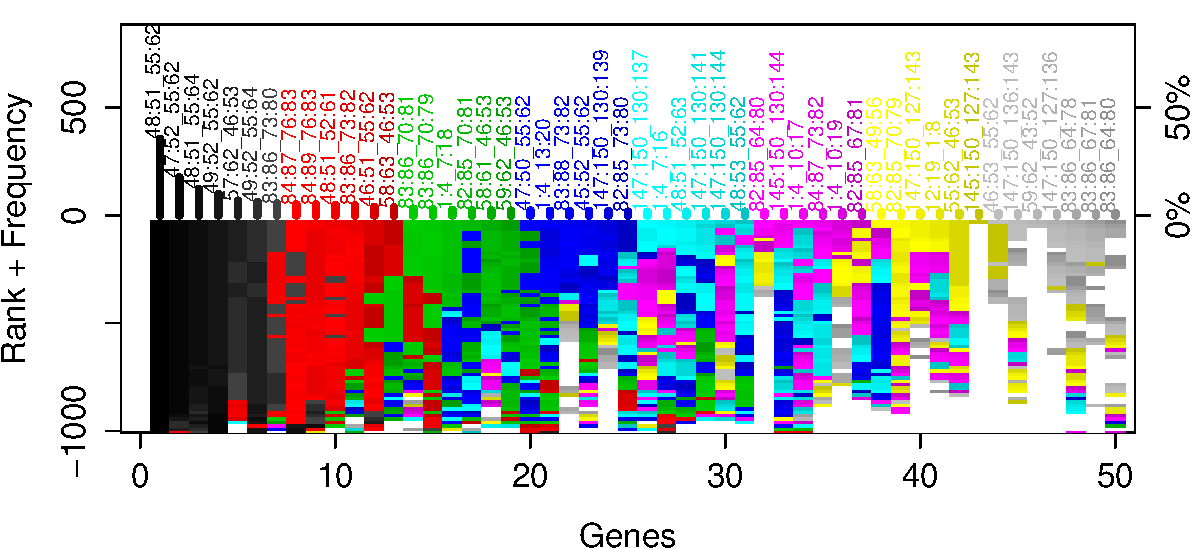
\includegraphics[width=10cm]{figs/ga_t_stab_crp.pdf}
\caption{Gene rank stability to predict $T_{eff}$ with the NC fitness
  function}
\label{fig:chr-stab}
 \end{center}
\end{figure}

The GA procedure provides us with a large collection of chromosomes,
and it is not clear which one should be chosen for the construction of
the regression model. In this work we adopt the strategy of using the
frequency of genes in the population of chromosomes as criteria for
inclusion in a forward selection strategy that eventually decides on
the optimal feature set as the one with the highest classification
accuracy with the lowest number of genes. {\bf I do not understand
  this. What you do is simply add features until one more feature does
  not improve the regression performance?}. In the case of the \teff
prediction model, this results in the features listed in
Table~\ref{tab:tab_NC_T}.

\begin{table}
\begin{center}
\begin{tabular}{rrrrr}
  \hline
 & Signal\_from & Signal\_To & Cont\_From & Cont\_To \\ 
  \hline
Feature 1 & 8451.60 & 8458.80 & 8473.20 & 8509.20 \\ 
Feature 2 & 8620.80 & 8628.00 & 8646.00 & 8667.60 \\ 
Feature 3 & 8653.20 & 8667.60 & 8613.60 & 8635.20 \\ 
Feature 4 & 8746.80 & 8754.00 & 8710.80 & 8739.60 \\ 
Feature 5 & 8977.20 & 8984.40 & 8916.00 & 8937.60 \\ 
   \hline
\end{tabular}
\caption {Recommended features and continuum bands for predicting
  $T_{eff}$ as evaluated using NC fitness
  function} \label{tab:tab_NC_T}
\end{center}
\end{table}


\cite{2013A&A...549A.129C} provide a set of features based on sensitivity 
maps that we collect in Table~\ref{tab:tab_cesetti} to facilitate
comparison with our proposal.


\begin{table}
\begin{center}
\begin{tabular}{rrrrrrr}
  \hline
 & Signal\_from & Signal\_To & Cont1\_From & Cont1\_To & Cont2\_From & Cont2\_To \\ 
  \hline
Pa1 & 8462.40 & 8473.20 & 8476.80 & 8484.00 & 8563.20 & 8574.00 \\ 
  Ca1 & 8484.00 & 8512.80 & 8476.80 & 8484.00 & 8563.20 & 8574.00 \\ 
  Ca2 & 8523.60 & 8559.60 & 8476.80 & 8484.00 & 8563.20 & 8574.00 \\ 
  Pa2 & 8577.60 & 8617.20 & 8563.20 & 8574.00 & 8620.80 & 8638.80 \\ 
  Ca3 & 8642.40 & 8682.00 & 8620.80 & 8638.80 & 8700.00 & 8721.60 \\ 
  Pa3 & 8732.40 & 8772.00 & 8700.00 & 8721.60 & 8779.20 & 8790.00 \\ 
  Mg & 8804.40 & 8808.00 & 8779.20 & 8790.00 & 8815.20 & 8847.60 \\ 
  Pa4 & 8851.20 & 8887.20 & 8815.20 & 8847.60 & 8890.80 & 8898.00 \\ 
   \hline
\end{tabular}
\caption {Recommended features and Continuum bandpass recommended in 
   \cite{2013A&A...549A.129C} as relevant for temperature}
   \label{tab:tab_cesetti} 
\end{center}
\end{table}



% Gravity

In regards with the Gravity, the GA recommends the features 
presentend in Table~\ref{tab:tab_NC_G}

\begin{table}
\begin{center}
\begin{tabular}{rrrrr}
  \hline
 & Signal\_from & Signal\_To & Cont\_From & Cont\_To \\ 
  \hline
Feature 1 & 8462.40 & 8476.80 & 8484.00 & 8520.00 \\ 
Feature 2 & 8620.80 & 8628.00 & 8667.60 & 8703.60 \\ 
Feature 3 & 8646.00 & 8653.20 & 8689.20 & 8710.80 \\ 
Feature 4 & 8656.80 & 8664.00 & 8689.20 & 8718.00 \\ 
Feature 5 & 8782.80 & 8790.00 & 8797.20 & 8818.80 \\ 
   \hline
\end{tabular}
\caption {Recommended features and Continuum bandpass for predicting $log(g)$ 
      by using NC fitness function} \label{tab:tab_NC_G} 
\end{center}
\end{table}

% Metallicity


Finally, features suggested for metallicity 
can be found in Table~\ref{tab:tab_NC_M}.

\begin{table}
\begin{center}
\begin{tabular}{rrrrr}
  \hline
 & Signal\_from & Signal\_To & Cont\_From & Cont\_To \\ 
  \hline
Feature 1 & 8516.40 & 8538.00 & 8548.80 & 8577.60 \\ 
Feature 2 & 8620.80 & 8628.00 & 8635.20 & 8671.20 \\ 
Feature 3 & 8782.80 & 8790.00 & 8797.20 & 8818.80 \\ 
Feature 4 & 8970.00 & 8977.20 & 8916.00 & 8952.00 \\ 
Feature 5 & 9009.60 & 9016.80 & 8980.80 & 9002.40 \\ 
   \hline
\end{tabular}
\caption {Recommended features and Continuum bandpass for predicting $Metallicity$ 
      by using NC fitness function} \label{tab:tab_NC_M} 
\end{center}
\end{table}


}


{\bf To be done by me, Luis: describe the wavelength ranges obtained
  in terms of known lines and compare with Cesetti.}

